\documentclass[10pt]{article}
%Formato extenso:report
\begin{sloppypar}
	
\end{sloppypar}
%Formato corto:article

% Esto es para que el LaTeX sepa que el texto esten espanol:
\usepackage[english]{babel}

\usepackage{amsmath, amsthm, amsfonts,amssymb}

% Borrame si quieres:
\usepackage{multicol}

% Referencias
\usepackage{hyperref}

% Paquete para escribir codigo
\usepackage{listings}
\lstset{basicstyle=\footnotesize\ttfamily,breaklines=true}
\usepackage{alltt}

% Paquete para incluir imagenes
\usepackage{graphicx}

% Paquete para incluir varias imagenes en una
\usepackage{subfig}

% para poder fijare las imagenes ([H])
\usepackage{float}

% para agregar opciones al enumerate
\usepackage{enumerate}

% Teoremas
\newtheorem{thm}{Teorema}[section]
\newtheorem{cor}[thm]{Corolario}
\newtheorem{lem}[thm]{Lema}
\newtheorem{prop}[thm]{Proposici\'on}
\theoremstyle{definition}
\newtheorem{defn}[thm]{Definici\'on}
\theoremstyle{remark}
\newtheorem{rem}[thm]{Observaci\'on}
\theoremstyle{definition}
\newtheorem{prob}{Problema}
\numberwithin{equation}{prob}

% Calculus symbols
\newcommand{\pd}[2]{\frac{\partial #1}{ \partial #2}}   % First partial derivative command
\newcommand{\td}[2]{\frac{\mathrm{d} #1}{ \mathrm{d} #2}}
\newcommand{\pdd}[2]{\frac{\partial^2 #1}{ \partial #2 ^2}}   % Second partial derivative command
\newcommand{\pddc}[3]{\frac{\partial^2 #1}{ \partial #2 \partial #3}}   % Second partial derivative command

% Continuum mechanics & FEM symbols
\def\sca   #1{\mbox{\rm{#1}}{}}
\def\mat   #1{\mbox{\boldmath $\mathsf #1$}}
\def\vec   #1{\mbox{\boldmath $#1$}{}}
\def\ten   #1{\mbox{\boldmath $#1$}{}}
\def\ltr   #1{\mbox{\sf{#1}}}
\def\bltr  #1{\mbox{\sffamily{\bfseries{{#1}}}}}

% math operators and symbols
\DeclareMathOperator{\dive}{div}
\DeclareMathOperator{\trace}{trace}
\DeclareMathOperator{\tr}{tr}
\DeclareMathOperator{\symm}{symm}
\DeclareMathOperator{\sk}{skew}
\DeclareMathOperator{\grad}{grad}
\DeclareMathOperator{\Grad}{Grad}
\DeclareMathOperator{\curl}{curl}
\DeclareMathOperator{\Curl}{Curl}
\def\R{\mbox{\(\mathbb{R}\)}}
\def\dx{\mbox{\(\,\mathrm{d}x\)}}

% Page margins
%\topmargin=-2cm
%\textheight=22cm
%\textwidth=17cm
%\oddsidemargin=0cm
\usepackage{geometry}
\geometry{left=2.5cm, right=2.5cm, top=2cm, bottom=3cm}

\usepackage{makeidx}
\makeindex


\begin{document}
	
	\begin{titlepage}
		
		
		%%%%% NO MOFIFICAR
		\begin{figure}
			\begin{minipage}{4cm}
				
\includegraphics[width=0.9\textwidth]{./figures/logo}
			\end{minipage}
			\begin{minipage}{11cm}
				\vspace{4mm}
				{\sc UNIVERSIDAD DE VALPARAÍSO}\\
				Escuela de Ingeniería Civil Biomédica\\
				{\bf CBM414 Procesamiento digital de señales biomédicas}\\
				\vspace{0mm}
				\hrulefill
			\end{minipage}
		\end{figure}
		\phantom{""}\vspace{60mm}
		
		
		%%%%% MODIFICAR
		\begin{center}
			\Huge{\textbf{Laboratory 2}}\vspace{95mm}\\
			\raggedleft \Large{Maximiliano Antonio Gaete Pizarro}\\ 
		\end{center}
		
		
	\end{titlepage}
	
\printindex


\section{Problem 1}

\subsection{Signal Definition}

We propose a signal composed of \( N = 5 \) cosines with different frequencies \( f_n \) in the range \( 1 < f_n < 50 \, \text{Hz} \). The selected frequencies are:
\[
f_0 = 6 \, \text{Hz}, \quad f_1 = 14 \, \text{Hz}, \quad f_2 = 22 \, \text{Hz}, \quad f_3 = 33 \, \text{Hz}, \quad f_4 = 45 \, \text{Hz}
\]
The signal is defined as:
\[
x(t) = \sum_{n=0}^{4} \cos(2 \pi f_n t)
\]
with \( f_{\text{max}} = 45 \, \text{Hz} \).

\subsection{Python Code}

\begin{lstlisting}[language=Python, caption=Definition of the composite signal]
import numpy as np
import matplotlib.pylab as plt

# Time interval
t0, t1 = 0, 1

# Define frequencies
f0, f1, f2, f3, f4 = 6, 14, 22, 33, 45
f_max = max(f0, f1, f2, f3, f4)

# Signal with 5 cosines
fs1 = 512  # High sampling rate
t1 = np.linspace(t0, t1, int(fs1), endpoint=False)
signal1 = np.cos(2*np.pi*f0*t1) + np.cos(2*np.pi*f1*t1) + np.cos(2*np.pi*f2*t1) + np.cos(2*np.pi*f3*t1) + np.cos(2*np.pi*f4*t1)
\end{lstlisting}

% Sección con las gráficas de los casos

\subsection{Requested Plots}

\subsubsection{Case 1: \( f_s \gg 2f_{\text{max}} \)}

\begin{figure}[H]
    \centering
    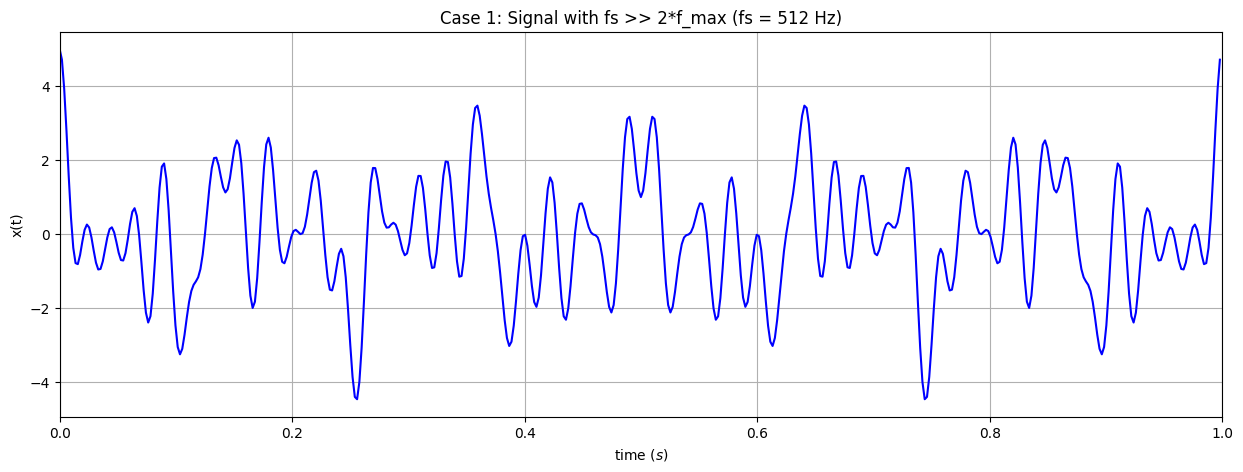
\includegraphics[width=\textwidth]{figures/output.png}
    \caption{Signal with \( f_s1 = 512 \, \text{Hz} \)}
    \label{fig:case1}
\end{figure}

\begin{lstlisting}[language=Python, caption=Case 1 - High sampling rate]
plt.figure(figsize=(15, 5))
plt.plot(t1, signal1)
plt.title(f'Case 1: Signal with fs >> 2*f_max (fs = {fs1} Hz)')
plt.xlabel("Time (s)")
plt.ylabel("x(t)")
plt.grid()
plt.show()
\end{lstlisting}

\subsubsection{Case 2: \( f_s = 2f_{\text{max}} \)}

\begin{figure}[H]
    \centering
    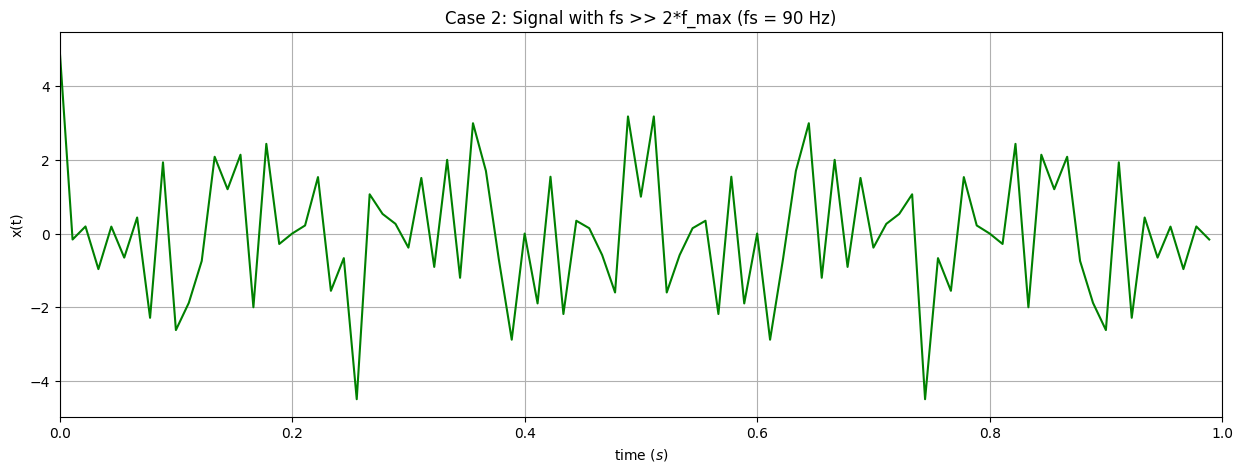
\includegraphics[width=\textwidth]{figures/output2.png}
    \caption{Signal with \( f_s2 = 90 \, \text{Hz} \)}
    \label{fig:case2}
\end{figure}

\begin{lstlisting}[language=Python, caption=Case 2 - Nyquist rate sampling]
fs2 = 2 * f_max  # fs2 = 2*f_max
t2 = np.linspace(t0, t1, int(fs2), endpoint=False)
signal2 = np.cos(2*np.pi*f0*t2) + np.cos(2*np.pi*f1*t2) + np.cos(2*np.pi*f2*t2) + np.cos(2*np.pi*f3*t2) + np.cos(2*np.pi*f4*t2)

plt.figure(figsize=(15, 5))
plt.plot(t2, signal2)
plt.title(f'Case 2: Signal with fs = 2*f_max (fs = {fs2} Hz)')
plt.xlabel("Time (s)")
plt.ylabel("x(t)")
plt.grid()
plt.show()
\end{lstlisting}

\subsubsection{Case 3: \( 0 < f_s \ll 2f_{\text{max}} \)}

\begin{figure}[H]
    \centering
    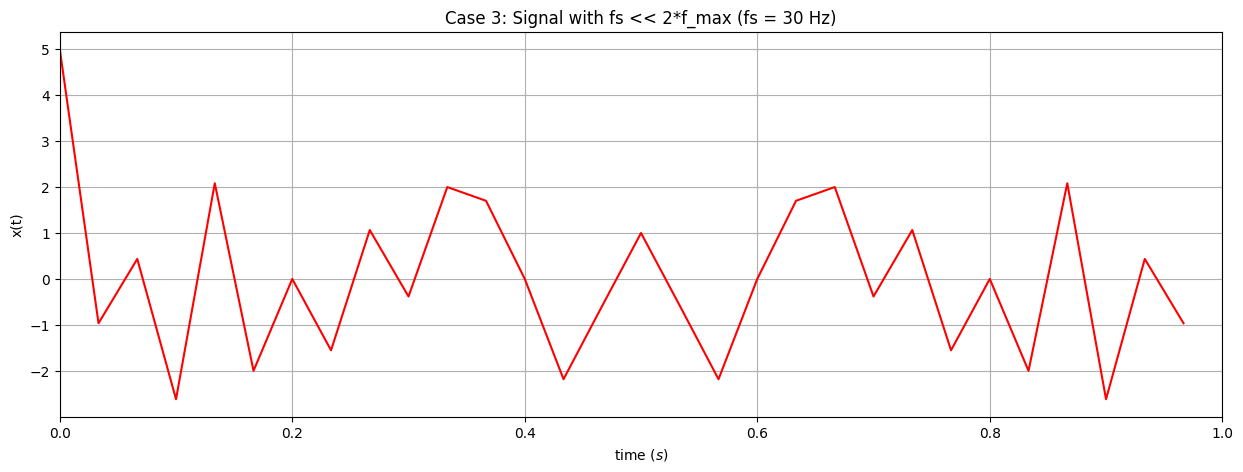
\includegraphics[width=\textwidth]{figures/output3.png}
    \caption{Signal with \( f_s3 = 30 \, \text{Hz} \)}
    \label{fig:case3}
\end{figure}

\begin{lstlisting}[language=Python, caption=Case 3 - Low sampling rate (aliasing)]
fs3 = 30  # fs3 << 2*f_max
t3 = np.linspace(t0, t1, int(fs3), endpoint=False)
signal3 = np.cos(2*np.pi*f0*t3) + np.cos(2*np.pi*f1*t3) + np.cos(2*np.pi*f2*t3) + np.cos(2*np.pi*f3*t3) + np.cos(2*np.pi*f4*t3)

plt.figure(figsize=(15, 5))
plt.plot(t3, signal3)
plt.title(f'Case 3: Signal with fs << 2*f_max (fs = {fs3} Hz)')
plt.xlabel("Time (s)")
plt.ylabel("x(t)")
plt.grid()
plt.show()
\end{lstlisting}

\subsubsection{Case 4: \( f_s = f_{\text{max}} \)}

\begin{figure}[H]
    \centering
    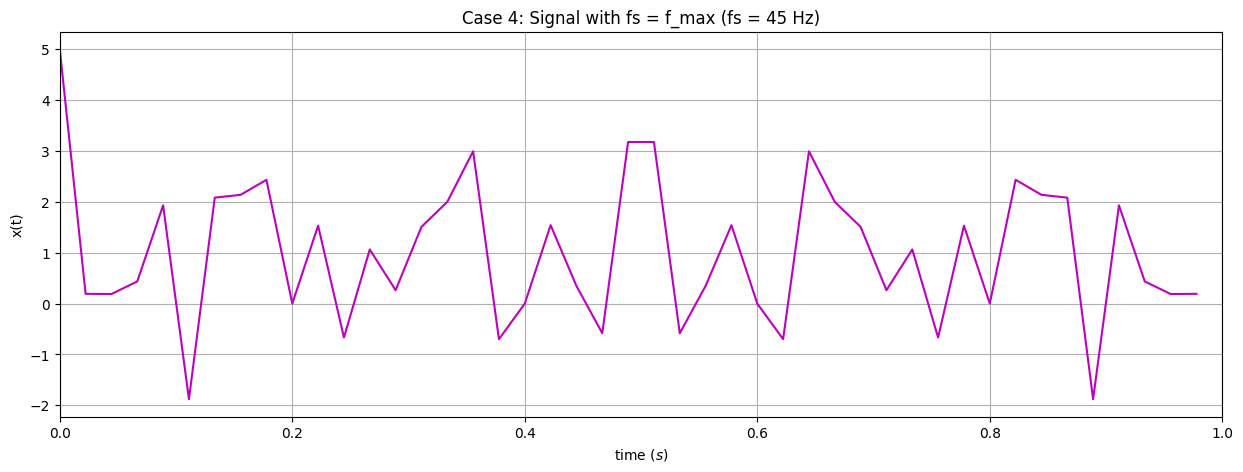
\includegraphics[width=\textwidth]{figures/output4.png}
    \caption{Signal with \( f_s4 = 45 \, \text{Hz} \)}
    \label{fig:case4}
\end{figure}

\begin{lstlisting}[language=Python, caption=Case 4 - Sampling at maximum frequency]
fs4 = f_max  # fs4 = f_max
t4 = np.linspace(t0, t1, int(fs4), endpoint=False)
signal4 = np.cos(2*np.pi*f0*t4) + np.cos(2*np.pi*f1*t4) + np.cos(2*np.pi*f2*t4) + np.cos(2*np.pi*f3*t4) + np.cos(2*np.pi*f4*t4)

plt.figure(figsize=(15, 5))
plt.plot(t4, signal4)
plt.title(f'Case 4: Signal with fs = f_max (fs = {fs4} Hz)')
plt.xlabel("Time (s)")
plt.ylabel("x(t)")
plt.grid()
plt.show()
\end{lstlisting}

\subsection{Alias Frequency Calculations}

\[
f_{\text{alias}} = \left| f - \left( \left\lfloor \frac{f}{f_s} + 0.5 \right\rfloor \cdot f_s \right) \right|
\]

The following alias frequencies were calculated for \( f_s3 = 30 \, \text{Hz} \) and \( f_s4 = 45 \, \text{Hz} \).

\begin{lstlisting}[language=Python, caption=Alias frequency calculation]
# Function to calculate alias frequency
def calculate_alias_frequency(f, fs):
    return np.abs(f - np.round(f / fs) * fs)

# Calculate alias frequencies for case 3 and 4
alias_f0_case3 = calculate_alias_frequency(f0, fs3)
alias_f1_case3 = calculate_alias_frequency(f1, fs3)
alias_f2_case3 = calculate_alias_frequency(f2, fs3)
alias_f3_case3 = calculate_alias_frequency(f3, fs3)
alias_f4_case3 = calculate_alias_frequency(f4, fs3)

alias_f0_case4 = calculate_alias_frequency(f0, fs4)
alias_f1_case4 = calculate_alias_frequency(f1, fs4)
alias_f2_case4 = calculate_alias_frequency(f2, fs4)
alias_f3_case4 = calculate_alias_frequency(f3, fs4)
alias_f4_case4 = calculate_alias_frequency(f4, fs4)
\end{lstlisting}

\subsection{Superimposed Plot of the Aliased Components}

\begin{figure}[H]
    \centering
    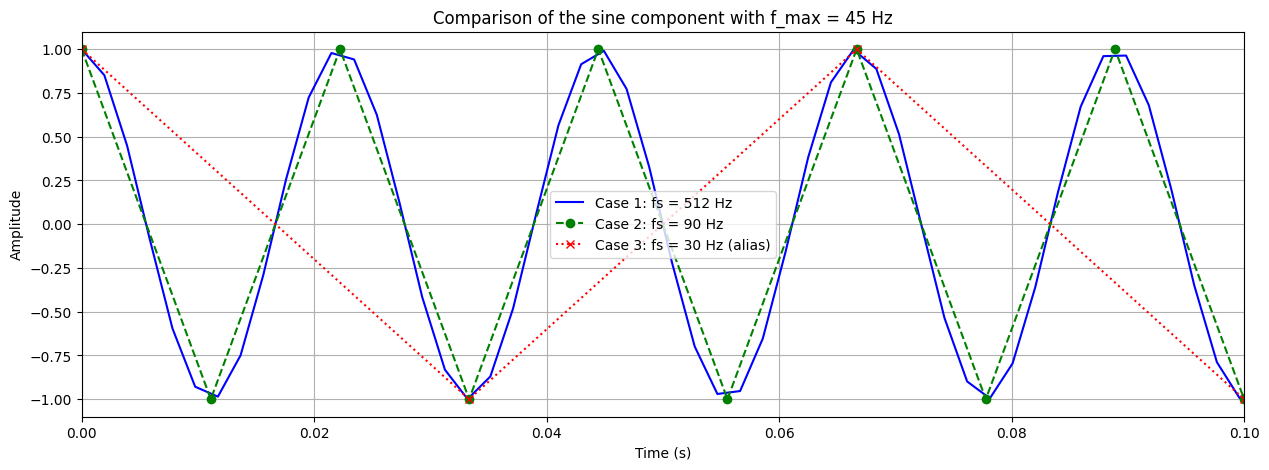
\includegraphics[width=\textwidth]{figures/output6.png}
    \caption{Comparison of the aliased components in \( f_s3 \) and \( f_s4 \)}
    \label{fig:comparison}
\end{figure}

\subsection{Final Analysis}

Aliasing occurs when the sampling frequency is less than \( 2f_{\text{max}} \), causing distorted signals during reconstruction. In Case 3, with \( f_s = 30 \, \text{Hz} \), we observe that the aliased frequencies produce low-frequency components that did not exist in the original signal. Similarly, in Case 4, with \( f_s = 45 \, \text{Hz} \), some components alias significantly (for example, \( f_4 \) aliases to \( 0 \, \text{Hz} \), meaning it disappears).

In conclusion, to avoid aliasing, it is crucial to sample the signal at a frequency greater than or equal to \( 2f_{\text{max}} \). Cases where \( f_s \) is less than \( 2f_{\text{max}} \) result in aliasing, which distorts the integrity of the original signal.

\section{Problem 2}

In this problem, we will analyze the frequency spectrum of the signal \( x(t) \) defined in Problem 1, using the same frequencies and number of cosines. We will generate the spectrum for different sampling frequencies and discuss how aliasing affects the results.

\subsubsection{Spectrum for \( f_s \gg 2f_{\text{max}} \)}

\begin{lstlisting}[language=Python]
import numpy as np
from scipy.fft import fft, fftfreq
import matplotlib.pylab as plt

# Frequencies and signal definition
f0, f1, f2, f3, f4 = 6, 14, 22, 33, 45
fs1 = 512  # Sampling frequency much greater than 2*f_max

t1 = np.linspace(0, 1, fs1, endpoint=False)
signal = np.cos(2*np.pi*f0*t1) + np.cos(2*np.pi*f1*t1) + np.cos(2*np.pi*f2*t1) + np.cos(2*np.pi*f3*t1) + np.cos(2*np.pi*f4*t1)

# FFT of the signal
yf = fft(signal)
xf = fftfreq(fs1, 1/fs1)[:fs1//2]

# Plot spectrum
plt.figure(figsize=(15, 5))
plt.plot(xf, 2.0/fs1 * np.abs(yf[:fs1//2]), color='b')
plt.title(f'Spectrum of the signal with fs >> 2*f_max (fs = {fs1} Hz)')
plt.xlabel('Frequency (Hz)')
plt.ylabel('Amplitude')
plt.grid()
plt.show()
\end{lstlisting}

\begin{figure}[H]
    \centering
    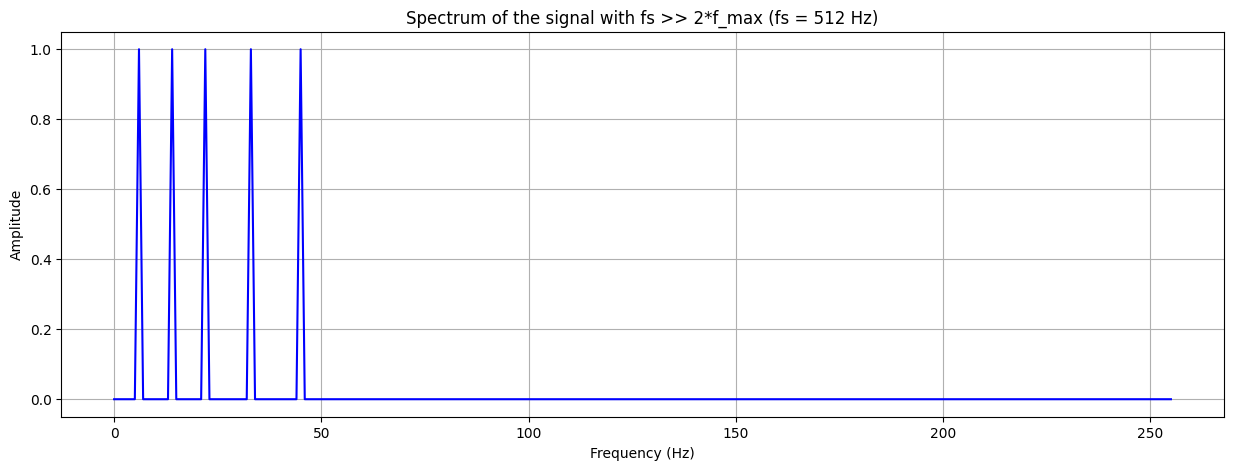
\includegraphics[width=\textwidth]{figures/output7.png}  
    \caption{Spectrum of the signal with \( f_s = 512 \, \text{Hz} \) (no aliasing).}
\end{figure}

\subsubsection{Spectrum for \( f_s = 2f_{\text{max}} \)}

\begin{lstlisting}[language=Python]
fs2 = 2 * f4  # Nyquist sampling frequency
t2 = np.linspace(0, 1, fs2, endpoint=False)
signal2 = np.cos(2*np.pi*f0*t2) + np.cos(2*np.pi*f1*t2) + np.cos(2*np.pi*f2*t2) + np.cos(2*np.pi*f3*t2) + np.cos(2*np.pi*f4*t2)

# FFT and spectrum
yf2 = fft(signal2)
xf2 = fftfreq(fs2, 1/fs2)[:fs2//2]

# Plot spectrum
plt.figure(figsize=(15, 5))
plt.plot(xf2, 2.0/fs2 * np.abs(yf2[:fs2//2]), color='g')
plt.title(f'Spectrum of the signal with fs = 2*f_max (fs = {fs2} Hz)')
plt.xlabel('Frequency (Hz)')
plt.ylabel('Amplitude')
plt.grid()
plt.show()
\end{lstlisting}

\begin{figure}[H]
    \centering
    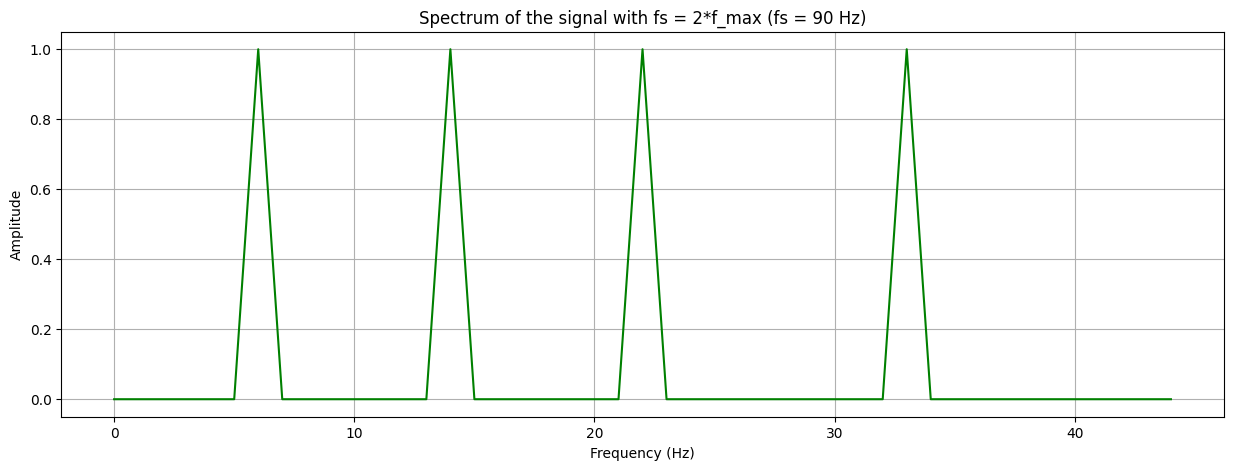
\includegraphics[width=\textwidth]{figures/output8.png}  
    \caption{Spectrum of the signal with \( f_s = 90 \, \text{Hz} \) (Nyquist rate).}
\end{figure}

\subsubsection{Spectrum for \( 0 < f_s \ll 2f_{\text{max}} \)}

\begin{lstlisting}[language=Python]
fs3 = 30  # Sampling frequency much lower than Nyquist rate
t3 = np.linspace(0, 1, fs3, endpoint=False)
signal3 = np.cos(2*np.pi*f0*t3) + np.cos(2*np.pi*f1*t3) + np.cos(2*np.pi*f2*t3) + np.cos(2*np.pi*f3*t3) + np.cos(2*np.pi*f4*t3)

# FFT and spectrum
yf3 = fft(signal3)
xf3 = fftfreq(fs3, 1/fs3)[:fs3//2]

# Plot spectrum
plt.figure(figsize=(15, 5))
plt.plot(xf3, 2.0/fs3 * np.abs(yf3[:fs3//2]), color='r')
plt.title(f'Spectrum of the signal with fs << 2*f_max (fs = {fs3} Hz)')
plt.xlabel('Frequency (Hz)')
plt.ylabel('Amplitude')
plt.grid()
plt.show()
\end{lstlisting}

\begin{figure}[H]
    \centering
    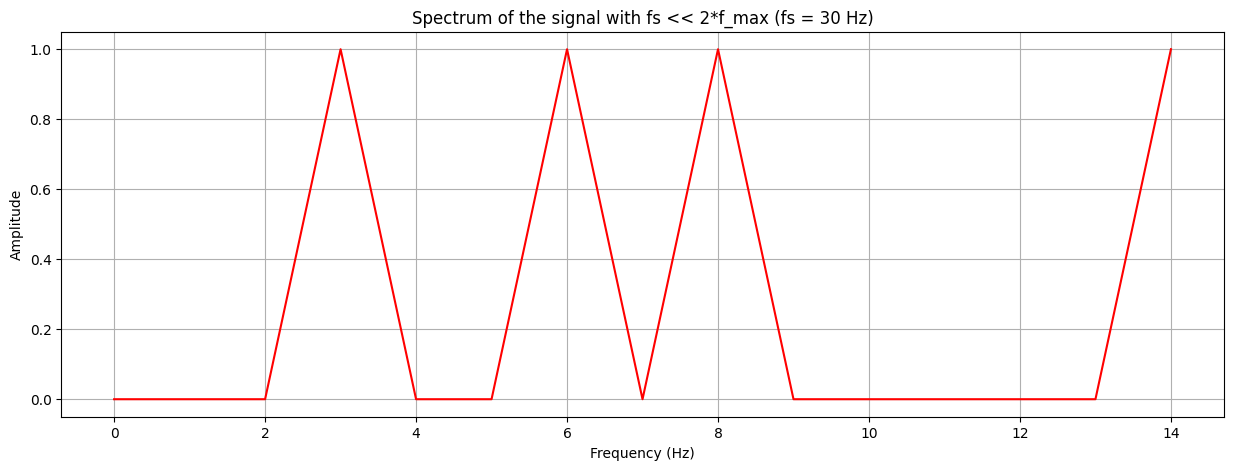
\includegraphics[width=\textwidth]{figures/output9.png}  
    \caption{Spectrum of the signal with \( f_s = 30 \, \text{Hz} \) (significant aliasing).}
\end{figure}

\subsubsection{Spectrum for \( f_s = f_{\text{max}} \)}

\begin{lstlisting}[language=Python]
fs4 = f4  # Sampling frequency equal to f_max
t4 = np.linspace(0, 1, fs4, endpoint=False)
signal4 = np.cos(2*np.pi*f0*t4) + np.cos(2*np.pi*f1*t4) + np.cos(2*np.pi*f2*t4) + np.cos(2*np.pi*f3*t4) + np.cos(2*np.pi*f4*t4)

# FFT and spectrum
yf4 = fft(signal4)
xf4 = fftfreq(fs4, 1/fs4)[:fs4//2]

# Plot spectrum
plt.figure(figsize=(15, 5))
plt.plot(xf4, 2.0/fs4 * np.abs(yf4[:fs4//2]), color='m')
plt.title(f'Spectrum of the signal with fs = f_max (fs = {fs4} Hz)')
plt.xlabel('Frequency (Hz)')
plt.ylabel('Amplitude')
plt.grid()
plt.show()
\end{lstlisting}

\begin{figure}[H]
    \centering
    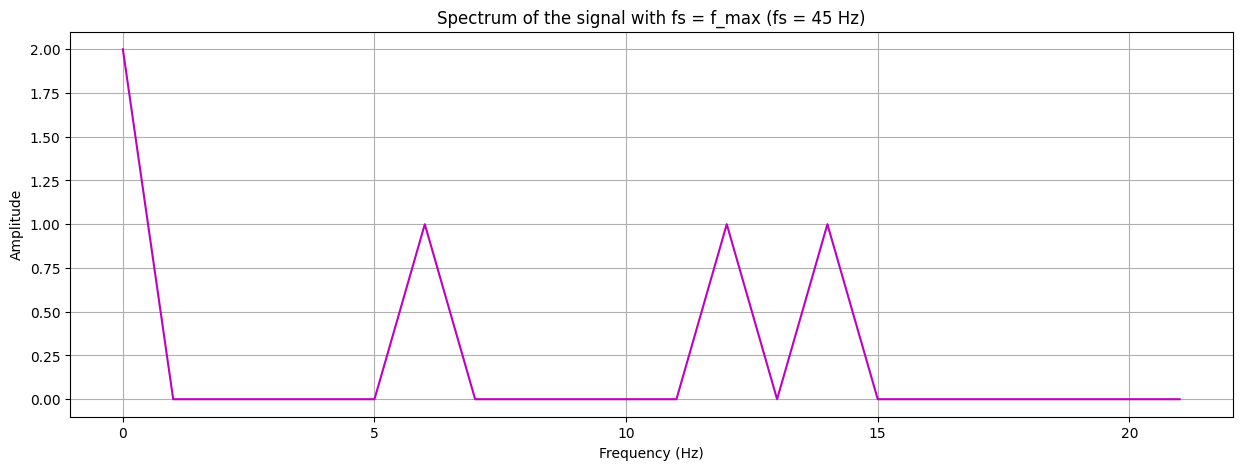
\includegraphics[width=\textwidth]{figures/output11.png}  
    \caption{Spectrum of the signal with \( f_s = 45 \, \text{Hz} \) (high aliasing).}
\end{figure}

\subsection{Formula \( f_a = f \mod (f_s) \)}

The formula \( f_a = f \mod (f_s) \) helps predict the position of aliasing components in the sampled spectrum. Essentially, this formula computes how a high-frequency component "folds" back into the lower frequency range if the sampling frequency is too low. In our spectra, we can see that the aliasing components follow this prediction.

\subsection{Analysis of the Spectra}

The frequency spectra generated in Parts 1 to 4 show how different sampling frequencies affect the signal. When the sampling frequency is greater than or equal to \( 2f_{\text{max}} \), the spectrum accurately captures the original frequency components. However, as the sampling frequency decreases below the Nyquist rate, aliasing becomes more prominent, and high-frequency components "fold" back into lower frequencies. These aliased components distort the spectrum and can result in incorrect interpretations of the signal content.

The choice of sampling frequency directly impacts the accuracy of the signal's frequency representation. To avoid aliasing, the sampling frequency must be at least twice the maximum frequency component present in the signal.

\section{Problem 3: ANALYSIS OF ALIASING IN A CHIRP SIGNAL}
In this problem, we analyze aliasing in a chirp signal, which is defined as a cosine function with a frequency that changes linearly over time. The general form of the chirp signal is given by:

\[
x(t) = \cos\left( 2\pi \phi(f_0, f_1; t) + \phi_0 \right), \quad t \in \mathbb{R}
\]

Where:
- \( f_0 \) is the initial frequency at \( t_0 \),
- \( f_1 \) is the final frequency at \( t_1 \),
- \( \phi_0 \) is the phase offset.

The phase function \( \phi(f_0, f_1; t) \) for a linear chirp is:

\[
\phi(f_0, f_1; t) = f_0 + (f_1 - f_0) \cdot \frac{t}{t_1}
\]

In this exercise, we consider the chirp signal with \( f_0 = 0 \, \text{Hz} \), \( f_1 = 50 \, \text{Hz} \), \( t_1 = 1 \, \text{s} \), and the number of samples \( N_{\text{sample}} = 512 \).

\subsection{Chirp Signal with \( f_s \gg 2f_1 \)}
We first plot the chirp signal and its spectrum for the case where the sampling frequency \( f_s \gg 2f_1 \). In this case, we use \( f_s = 512 \, \text{Hz} \), which is much higher than the Nyquist rate.

The following Python code generates the plot and the spectrum:

\begin{lstlisting}[language=Python]
import numpy as np
from scipy.fft import fft, fftfreq
import matplotlib.pylab as plt
from scipy import signal

# Signal chirp parameters definition
t0, t1 = 0, 1
f0, f1 = 0, 50
Nsample = 512

# Generation of the chirp signal for different sampling frequencies
def plot_chirp_and_spectrum(fs):
    t = np.linspace(t0, t1, int(Nsample * fs / 512), endpoint=False)
    chirp_signal = signal.chirp(t, f0, t1, f1, method='linear')

    # Plot of the chirp signal in time domain
    plt.figure()
    plt.plot(t, chirp_signal, color='b')
    plt.ylim(-1, 1)
    plt.xlabel(r"Time $(s)$", size=16)
    plt.ylabel(r"x(t)", size=16)
    plt.title(f'Chirp signal plot with $f_s = {fs}$ Hz', size=16)
    plt.grid()
    plt.tight_layout()
    plt.show()

    # FFT of the chirp signal
    yf = fft(chirp_signal)
    xf = fftfreq(len(chirp_signal), 1 / fs)[:len(chirp_signal) // 2]

    # Plot of the spectrum
    plt.figure()
    plt.plot(xf, 2.0 / len(chirp_signal) * np.abs(yf[:len(chirp_signal) // 2]), color='b')
    plt.title(f'Spectrum of the chirp signal with $f_s = {fs}$ Hz', size=16)
    plt.grid()
    plt.tight_layout()
    plt.show()

# Case: Sampling frequency fs >> 2f1
plot_chirp_and_spectrum(512)
\end{lstlisting}

\begin{figure}[H]
    \centering
    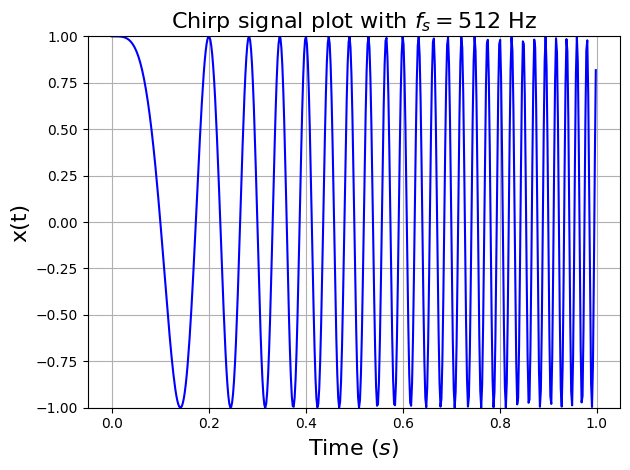
\includegraphics[width=\textwidth]{figures/output12.png}  
    \caption{Chirp signal with \( f_s = 512 \, \text{Hz} \).}
\end{figure}

\begin{figure}[H]
    \centering
    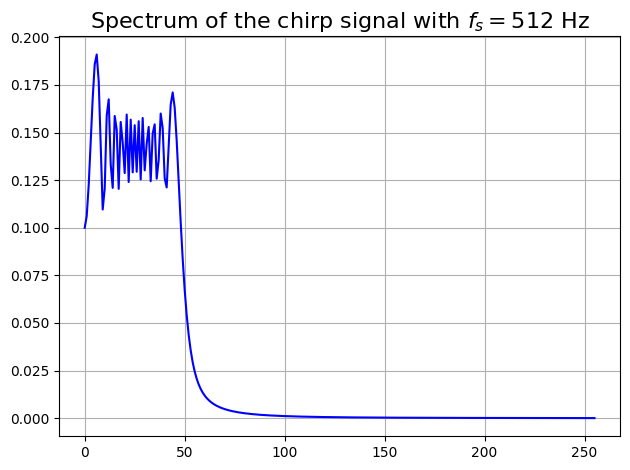
\includegraphics[width=\textwidth]{figures/output13.png}  
    \caption{Spectrum of the chirp signal with \( f_s = 512 \, \text{Hz} \).}
\end{figure}

\subsubsection{Chirp Signal with \( f_s = 2f_1 \)}
Next, we analyze the chirp signal with a sampling frequency \( f_s = 2f_1 \), which is equal to the Nyquist rate.

\begin{lstlisting}[language=Python]
# Case: Sampling frequency fs = 2f1
plot_chirp_and_spectrum(2 * f1)
\end{lstlisting}

\begin{figure}[H]
    \centering
    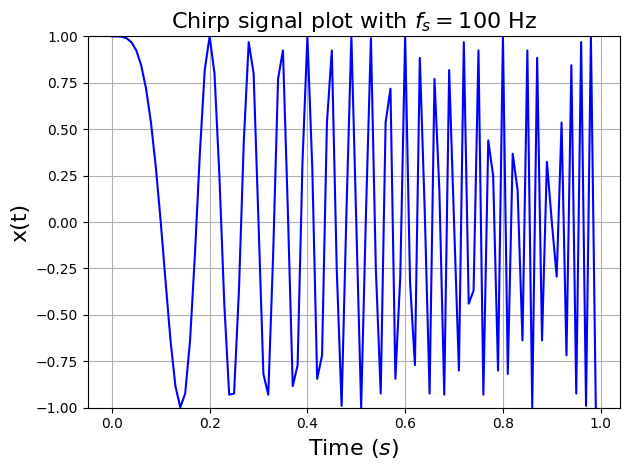
\includegraphics[width=\textwidth]{figures/output14.png} 
    \caption{Chirp signal with \( f_s = 100 \, \text{Hz} \) (Nyquist rate).}
\end{figure}

\begin{figure}[H]
    \centering
    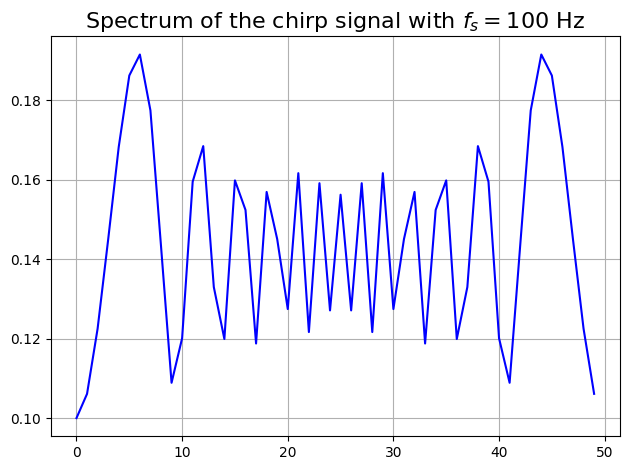
\includegraphics[width=\textwidth]{figures/output15.png}  
    \caption{Spectrum of the chirp signal with \( f_s = 100 \, \text{Hz} \).}
\end{figure}

\subsubsection{Chirp Signal with \( f_s = f_1 \)}
Finally, we plot the chirp signal and its spectrum for the case where the sampling frequency is equal to the final frequency \( f_1 \), i.e., \( f_s = f_1 \), which causes aliasing.

\begin{lstlisting}[language=Python]
# Case: Sampling frequency fs = f1
plot_chirp_and_spectrum(f1)
\end{lstlisting}

\begin{figure}[H]
    \centering
    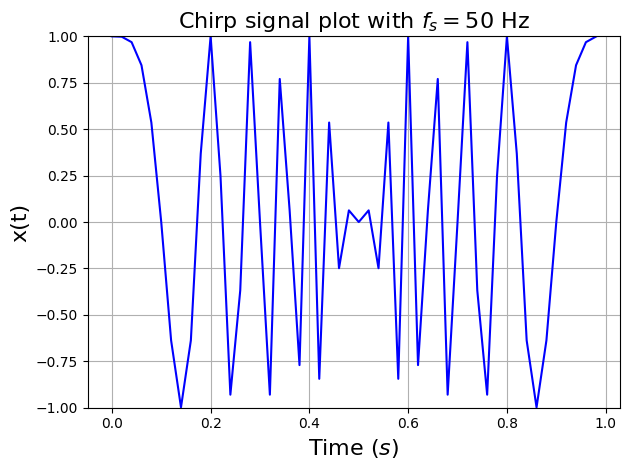
\includegraphics[width=\textwidth]{figures/output16.png}  
    \caption{Chirp signal with \( f_s = 50 \, \text{Hz} \) (aliasing).}
\end{figure}

\begin{figure}[H]
    \centering
    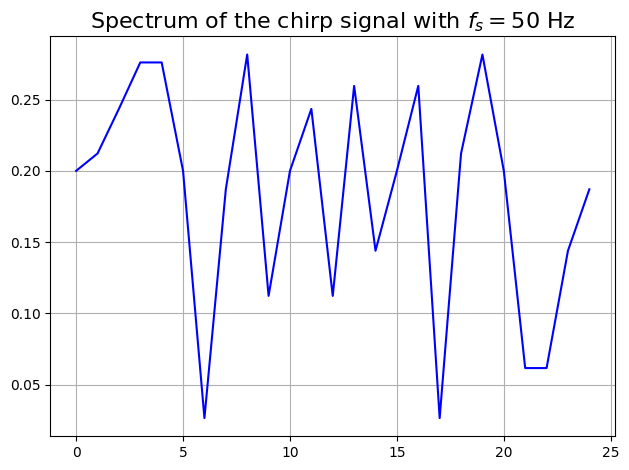
\includegraphics[width=\textwidth]{figures/output17.png}  
    \caption{Spectrum of the chirp signal with \( f_s = 50 \, \text{Hz} \).}
\end{figure}

\subsection{Analysis of Aliasing Effects}
In the first case, where the sampling frequency \( f_s \gg 2f_1 \), the chirp signal is sampled accurately without any distortion, and its frequency spectrum shows the original frequency components.

When \( f_s = 2f_1 \), we reach the Nyquist rate. At this point, the signal can still be reconstructed correctly, but the highest frequencies may experience some distortion, especially near the end of the time interval.

In the third case, where \( f_s = f_1 \), severe aliasing occurs. The sampling frequency is insufficient to capture the high-frequency components, which fold back into the lower frequencies, corrupting the signal. This is reflected in the spectrum, where we observe spurious peaks due to aliasing.



\section{Problem 4: Convolution}

Discrete convolution is a mathematical operation that combines two sequences (or signals) into a new sequence. Each element of the new sequence is a weighted sum of the products of the elements of the two original sequences. Formally, if \(x[n]\) and \(h[n]\) are two discrete sequences, their convolution \(y[n]\) is defined as:

\[
y[n] = (x * h)[n] = \sum_{k=-\infty}^{\infty} x[k] \cdot h[n-k]
\]

Where:
\begin{itemize}
    \item \(x[k]\) is the first sequence.
    \item \(h[n-k]\) is the second sequence shifted by \(k\) positions.
    \item The sum is performed over all values of \(k\), which means that each point of \(y[n]\) is the sum of the products of the corresponding values of \(x[k]\) and \(h[n-k]\).
\end{itemize}

The goal of this problem is to implement convolution using two different methods: a custom implementation and the FFT-based method provided by SciPy. The convolution will be performed on a square wave signal.

\subsection{Implementing Custom Convolution}

We define two signals: an unfiltered square wave (\textit{señal\_sin\_filtrar}) and a filter (\textit{filtro}) which is another square wave. The custom convolution function is implemented in Python as shown below:

\begin{lstlisting}[language=Python]
def custom_convolution(unfiltered_signal, filter_signal):
    """
    Performs the discrete convolution of two sequences x and h.
    Parameters:
    x: list or array, input sequence.
    h: list or array, impulse response (or filter sequence).
    Returns:
    y: list, result of the convolution.
    """
    Nx = len(unfiltered_signal)
    Nh = len(filter_signal)
    conv = np.zeros(Nx)
    for n in range(Nh):
        for k in range(Nx):
            conv[k] += unfiltered_signal[k-n] * filter_signal[n]
    return 1.0 / Nx * conv
\end{lstlisting}

The convolution of the square wave with the filter is computed using this custom function. The FFT-based convolution is also applied to compare the results. Below are the plots of the original signal, the convolution result, and the FFT-based convolution result.

\begin{figure}[H]
    \centering
    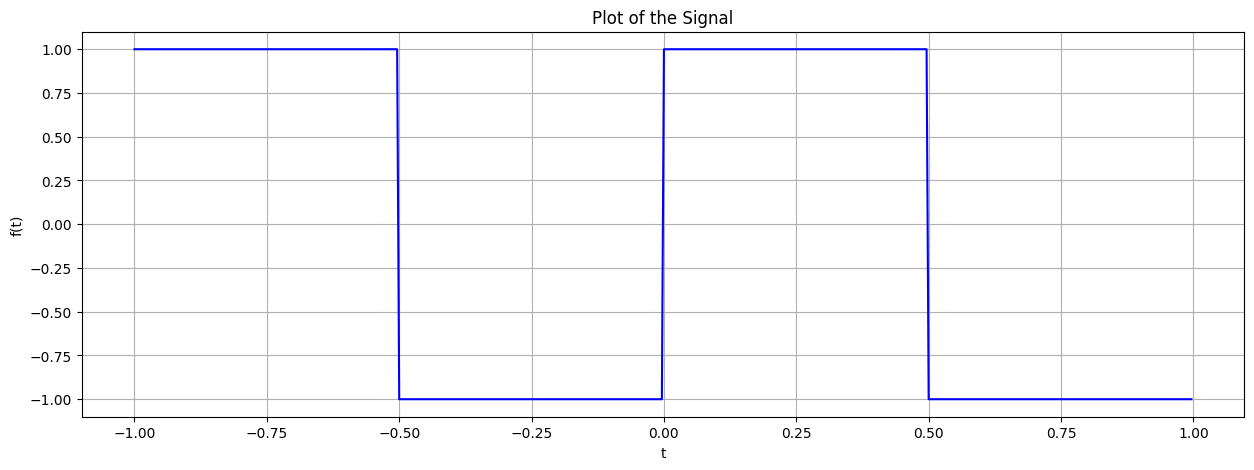
\includegraphics[width=\textwidth]{figures/output18.png}  % Replace with actual path
    \caption{Original square wave signal.}
\end{figure}

\begin{figure}[H]
    \centering
    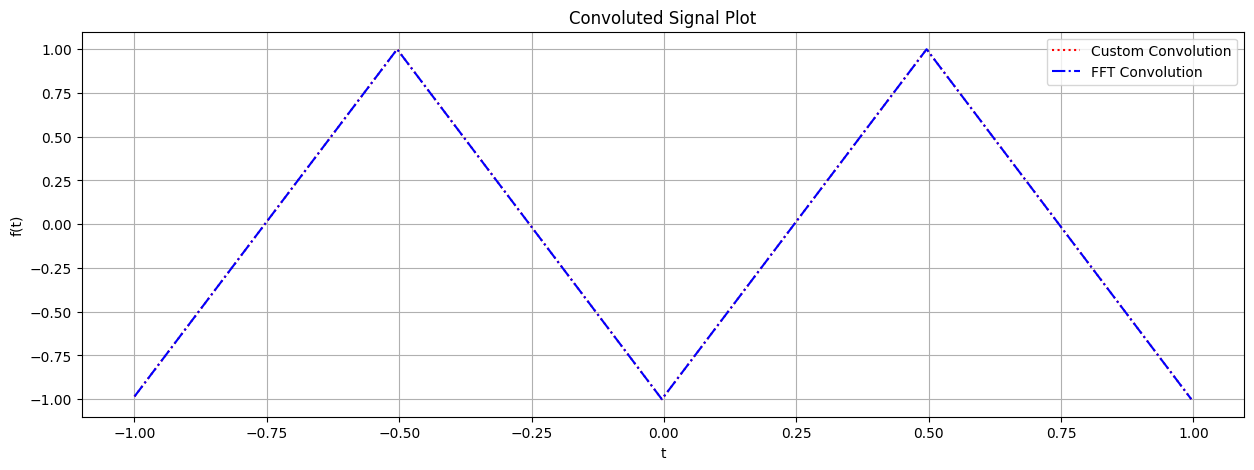
\includegraphics[width=\textwidth]{figures/output19.png}  % Replace with actual path
    \caption{Comparison of custom convolution and FFT-based convolution.}
\end{figure}

\subsection{Time Complexity Analysis}

To analyze the computational cost, we measure the time required to perform the convolution using both methods for \(N_{\text{sample}} = 512\). The timing results are obtained using the \texttt{timeit} function for both the custom convolution and the FFT-based convolution.

\begin{lstlisting}[language=Python]
import timeit

# Measure time using FFT
fft_time_512 = timeit.timeit(lambda: signal.convolve(scuad, fcuad, mode='same', method='fft'), number=500)
print(f"Time using FFT with Nsample=512: {fft_time_512} seconds")

# Measure time using direct method
direct_time_512 = timeit.timeit(lambda: signal.convolve(scuad, fcuad, mode='same', method='direct'), number=500)
print(f"Time using direct method with Nsample=512: {direct_time_512} seconds")
\end{lstlisting}

\begin{lstlisting}[language=Python]
# Measure time using FFT
fft_time_512 = 0.03657470000325702  # Measured time for FFT-based method
direct_time_512 = 0.016344199975719675  # Measured time for direct method
\end{lstlisting}

The timing results for \(N_{\text{sample}} = 512\) are as follows:
\begin{itemize}
    \item Time using FFT method: \(0.0365 \, \text{seconds}\)
    \item Time using direct method: \(0.0163 \, \text{seconds}\)
\end{itemize}
For this smaller sample size, the direct method outperforms the FFT-based method in terms of speed. This is expected because for smaller signals, the overhead of performing the FFT may outweigh the benefits of its \(O(N \log N)\) time complexity, compared to the direct method's \(O(N^2)\) time complexity.


\subsection{Using SciPy's \texttt{signal.convolve}}

We also utilize the \texttt{signal.convolve} function provided by SciPy to perform the convolution with two different methods: FFT-based and direct. The results are compared as follows:

\begin{lstlisting}[language=Python]
# FFT-based convolution
conv_fft = signal.convolve(scuad, fcuad, mode='same', method='fft')

# Direct convolution
conv_direct = signal.convolve(scuad, fcuad, mode='same', method='direct')

# Plot the results
plt.figure(figsize=(15, 5))
plt.plot(t, conv_fft, color='r', linestyle=':', label='Convolution (FFT)')
plt.plot(t, conv_direct, color='b', linestyle='-.', label='Convolution (Direct)')
plt.xlabel('t')
plt.ylabel('f(t)')
plt.title('Convolution of Signals')
plt.legend()
plt.grid()
plt.show()
\end{lstlisting}

\begin{figure}[H]
    \centering
    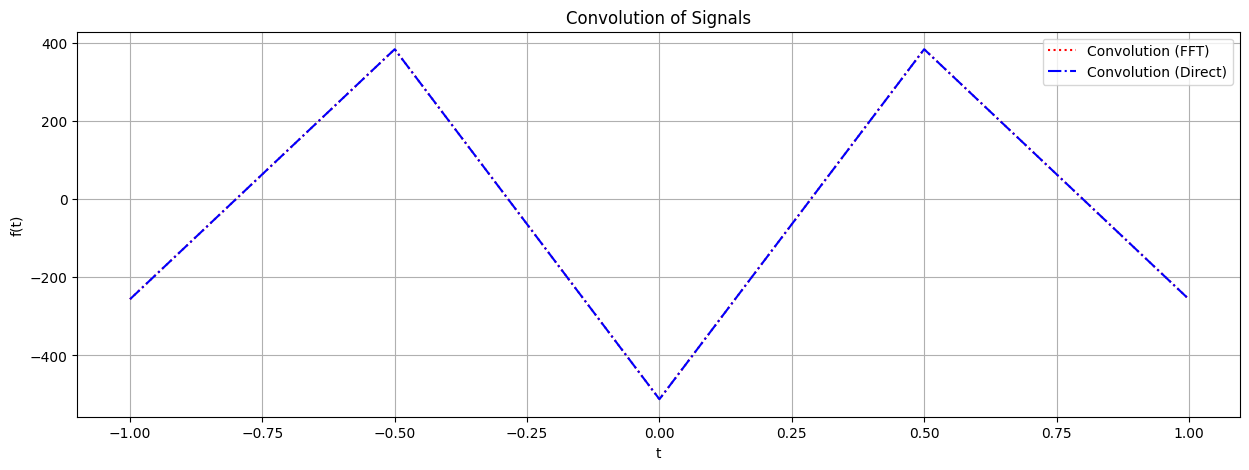
\includegraphics[width=\textwidth]{figures/output21.png}  % Replace with actual path
    \caption{Comparison of FFT-based convolution and direct convolution.}
\end{figure}

As observed in the plot, the results of both methods are similar, but the FFT-based method is more efficient for larger sequences.

\subsection{Increasing the Sample Size to \(N_{\text{sample}} = 5000\)}

Next, we increase the number of samples to \(N_{\text{sample}} = 5000\) and measure the time for both convolution methods.

\begin{lstlisting}[language=Python]
# Change the sample size
Nsample = 5000
t = np.linspace(-1, 1, Nsample, endpoint=False)

# Square wave signal and filter
scuad = square_wave_scipy(t, T)
fcuad = filter_square(t)

# Measure time using FFT
fft_time_5000 = timeit.timeit(lambda: signal.convolve(scuad, fcuad, mode='same', method='fft'), number=500)
print(f"Time using FFT with Nsample=5000: {fft_time_5000} seconds")

# Measure time using direct method
direct_time_5000 = timeit.timeit(lambda: signal.convolve(scuad, fcuad, mode='same', method='direct'), number=500)
print(f"Time using direct method with Nsample=5000: {direct_time_5000} seconds")
\end{lstlisting}

\begin{lstlisting}[language=Python]
# Change the sample size to 5000
fft_time_5000 = 0.10668810000061058  # Measured time for FFT-based method with Nsample=5000
direct_time_5000 = 1.2346499999985099  # Measured time for direct method with Nsample=5000
\end{lstlisting}

The timing results for \(N_{\text{sample}} = 5000\) are as follows:
\begin{itemize}
    \item Time using FFT method: \(0.1067 \, \text{seconds}\)
    \item Time using direct method: \(1.2346 \, \text{seconds}\)
\end{itemize}

For the larger sample size, the FFT-based method becomes significantly faster, while the direct method's time increases dramatically. This demonstrates the advantage of using FFT for larger signals, as its \(O(N \log N)\) time complexity becomes more efficient than the \(O(N^2)\) complexity of the direct method.


\subsection{Conclusion}

In this analysis, we compared the computation times of FFT-based convolution and direct convolution for two different sample sizes: \(N_{\text{sample}} = 512\) and \(N_{\text{sample}} = 5000\). For smaller signals, the direct method performed better. However, as the sample size increased, the FFT-based method became significantly more efficient. This highlights the importance of choosing the right method depending on the signal size. For large signals, FFT-based convolution is clearly the optimal choice in terms of computation time.

\section{Problem 5: Anti-aliasing filter}

\textbf{Find one or more definitions of the decibel unit (dB) and attenuation. You can use sources such as Wikipedia, ChatGPT, or any other online resource and write them exactly as they appear, whether they are in English or Spanish.}

\textbf{Definition of Decibel (dB):}

\textit{``The decibel (dB) is a logarithmic unit used to express the ratio of two values of a physical quantity, often power or intensity. One decibel is one-tenth of a bel, a rarely used unit. The decibel is used for a wide variety of measurements in science and engineering, most prominently in acoustics, electronics, and control theory. A decibel is one-tenth of a bel, where a bel represents a ratio of 10-to-1.''}
\textit{(Source: Wikipedia, ``Decibel'', en.wikipedia.org/wiki/Decibel)}\\

\textbf{Definition of Attenuation:}

\textit{``Attenuation is the gradual loss of flux intensity through a medium. In the case of signals, attenuation occurs when the strength of the signal reduces while it travels over distance or through obstacles, such as cables, fibers, or air. Attenuation is usually measured in decibels (dB) and indicates the reduction in strength.''}
\textit{(Source: Wikipedia, ``Attenuation'', en.wikipedia.org/wiki/Attenuation)}\\

\textbf{1. Interpretation of Decibel and Attenuation:}

A decibel (dB) is a unit that measures the relative intensity of power or amplitude between two signals, often used to compare sound or electronic signal levels. Attenuation refers to the decrease in signal strength as it passes through a medium, where the decibel is typically used to quantify this reduction.

\textbf{2. Analysis of Attenuation in the Magnitude Expression $| \cdot |$:}

In the magnitude expression $| \cdot |$, the division indicates the comparison between the initial signal strength and the reduced signal strength due to attenuation. The ratio is crucial in measuring how much the signal has weakened over a given distance or medium. From the definitions of decibel and attenuation, this division reflects the proportional loss measured in decibels. The frequency $f_0$ determines the base point of the signal in the analysis of its strength over different mediums. Attenuation is frequency-dependent, meaning the amount of attenuation might change as the frequency varies.

\end{document}